% !TEX encoding = cp1250
\chapter{Projekt}
Implementacja projektu znajduje si� w pliku pust\_projekt1.mlx.

\section{Sprawdzenie poprawno�ci warto�ci punktu pracy}

Symulowane warto�ci s� sta�e oraz zgodne z punktem pracy ($U_{pp}$, $V_{pp}$).

\begin{figure}[H]
	\centering
	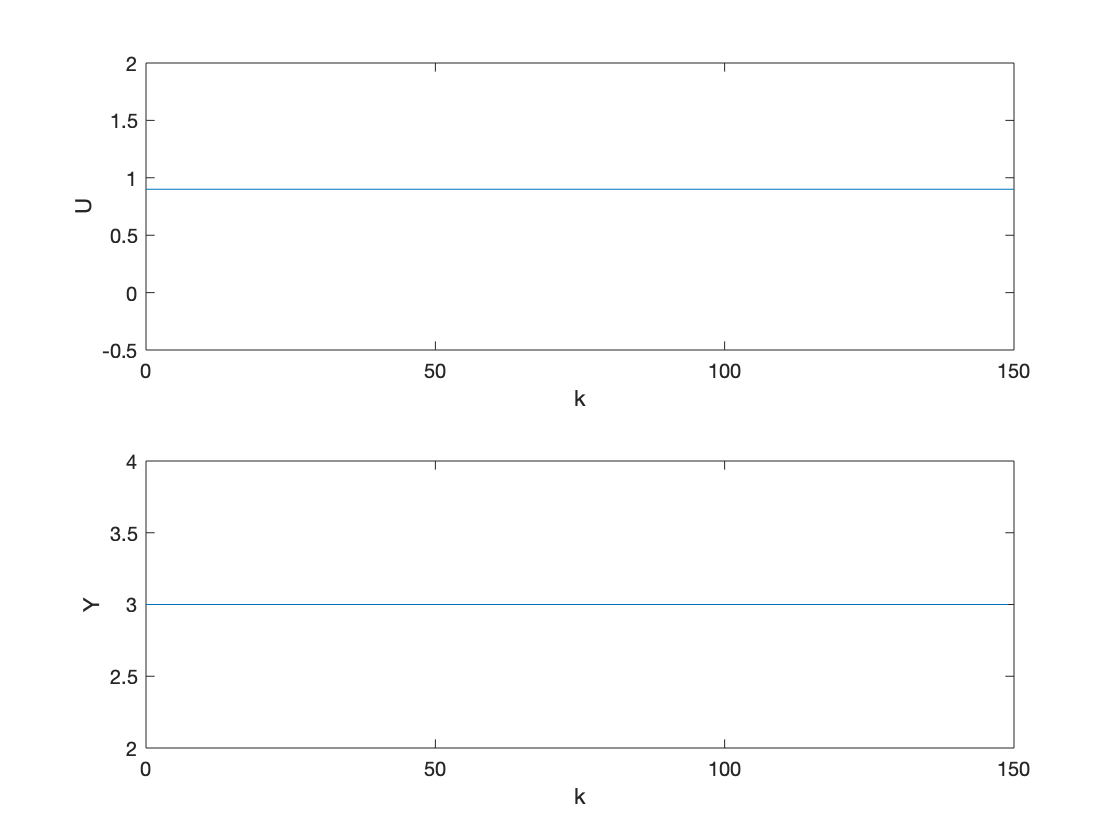
\includegraphics[scale=0.35]{png/pro_zad1.png}
	\caption{Warto�� zadana i wyj�cie w punkcie pracy}
	\label{rys_zad1}
\end{figure}

\section{Odpowiedzi skokowe procesu}

Obiekt zosta� pobudzony 4 r�nymi sygna�ami mieszcz�cymi si� w zakresie [$U_{min}$, $U_{max}$]. 
Zmiana sygna�u z $U_{pp}$ nast�pi�a w chwili k = 11. 

\begin{figure}[H]
	\centering
	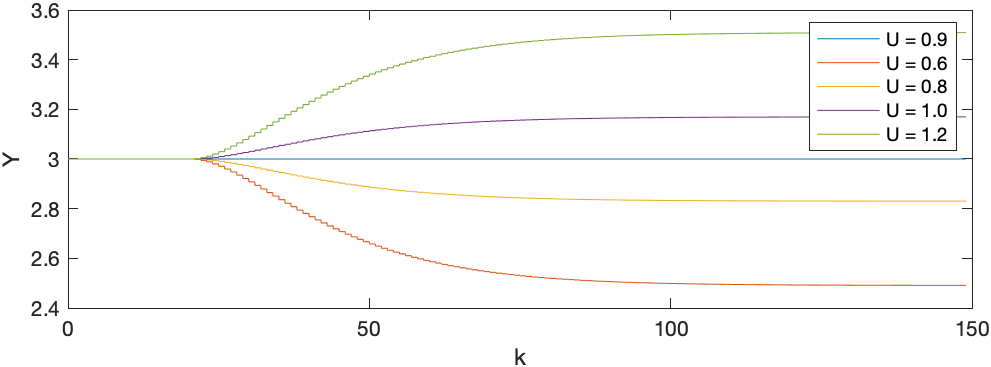
\includegraphics[scale=0.73]{png/pro_zad21.png}
	\caption{Odpowiedzi skokowe procesu}
	\label{rys_zad21}
\end{figure}

Na Rys. 2.3. naniesione zosta�y punkty (U, Y) dla ka�dego symulowanego pobudzenia.
Dopasowana prosta potwierdza w�a�ciwo�ci liniowe charakterystyki statycznej.

\begin{figure}[H]
	\centering
	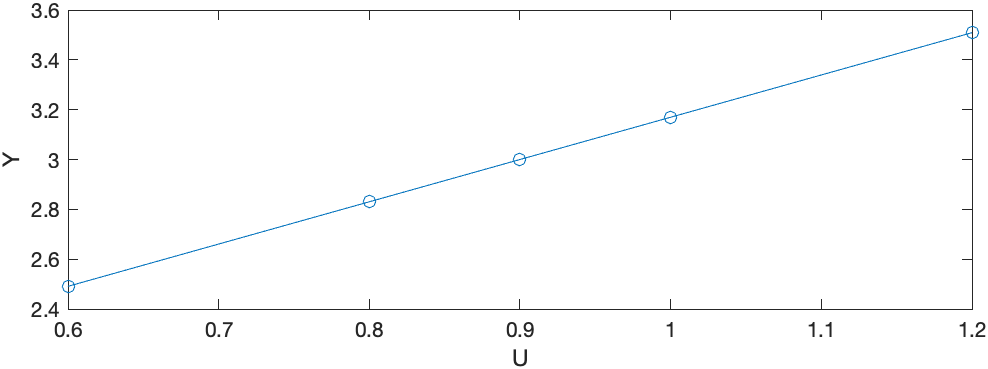
\includegraphics[scale=0.73]{png/pro_zad22.png}
	\caption{Charakterystyka statyczna}
	\label{rys_zad22}
\end{figure}

Wzmocnienie statyczne wyznaczone jest jako wsp�czynnik kierunkowy charaktetystyki 2.3.
\begin{align*}
K_{stat}=1.6966
\end{align*}


\section{Odpowied� skokowa w algorytmie DMC}
\section{Algorytm PID}

TO DO
Metoda Zieglera-Nicholsa - tabelka z obliczaniem nastaw.

\begin{table}
	[b] \caption{Regu�y Zieglera-Nicholsa (Z-N) wg cech przebiegu krytycznego (1942 r.)}
	\label{t_wyrownanie_do_znaku_przecinek3}
	\centering
	\sisetup{table-auto-round=true}
	\begin{small}
		\begin{tabular}{|l|S[table-format=2]|S[table-format=1.2]|S[table-format=1.2]|S[table-format=2.2]|S[table-format=2.2]|S[table-format=2.2]|S[table-format=3.2]|}
			\hline
			\multicolumn{1}{|c|}{Regulator\rule{0pt}{3.25mm}} & \hspace{0.5cm} $K$ \hspace{0.5cm} & ${T_i}$ & ${T_d}$  \\ \hline
			
			P\rule{0pt}{3.5mm} & ${0,5K_{kr}}$ & ${\infty}$  & ${0}$ \\ \hline
			
			PI\rule{0pt}{3.5mm} & ${0,45K_{kr}}$ & ${T_{kr}/1,2}$  & ${0}$  \\ \hline
			
			PID\rule{0pt}{3.5mm} & ${0,6K_{kr}}$  & ${0,5T_{kr}}$ & ${0,125T_{kr}}$  \\ \hline
			
		\end{tabular}
	\end{small}
\end{table}


Ti = inf, Td = 0 (regulator P) i stopniowo zwi�kszamy K �eby wywo�a� niegasn�ce oscylacje. 

%\begin{figure}[H]
%	\centering
%	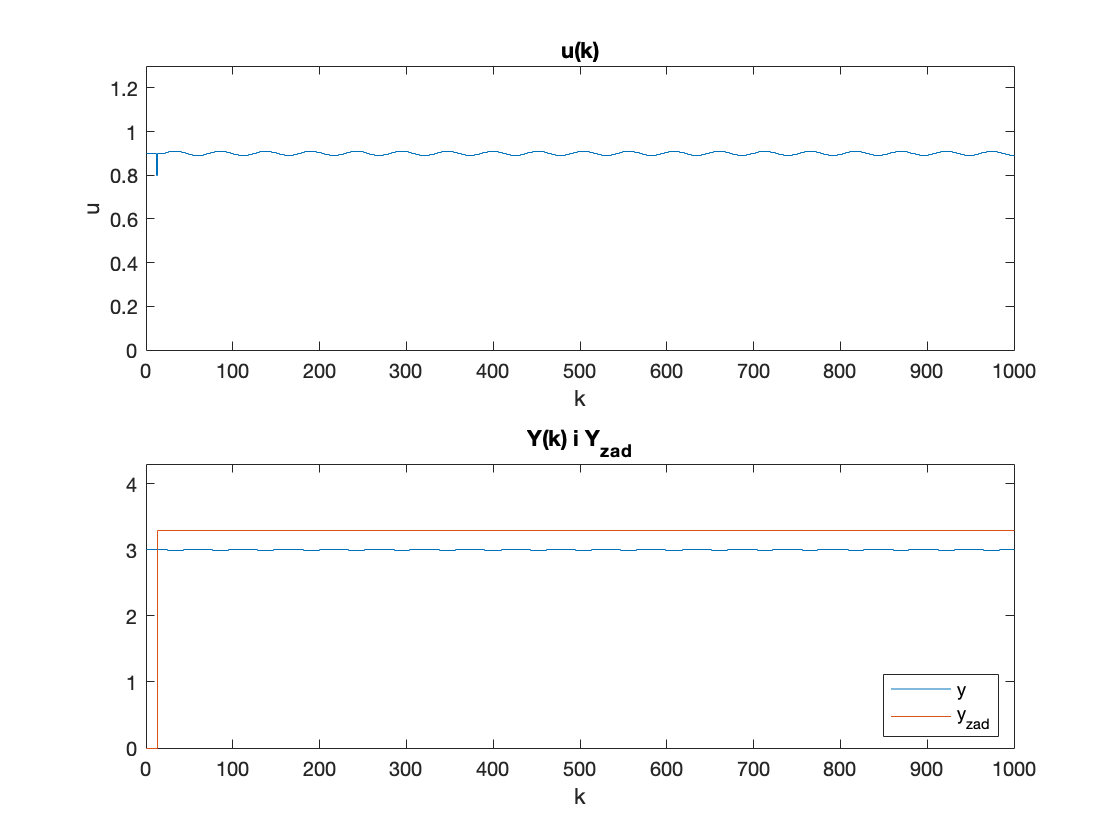
\includegraphics[scale=0.35]{png/pro_zad4_5_PID/pro1_PID_K_kryt.png}
%	\caption{Wyznaczenie K krytycznego}
%	\label{rys_przebiegi_T1}
%\end{figure}

\begin{figure}[H]
	\centering
	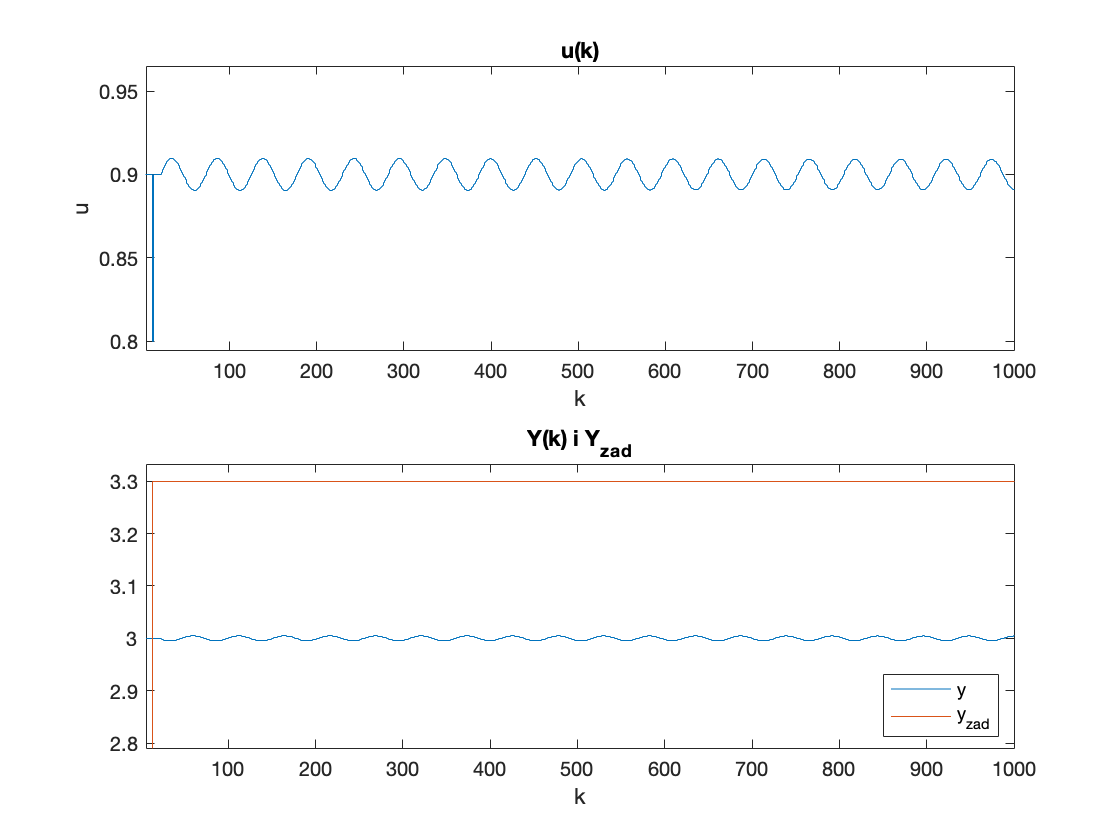
\includegraphics[scale=0.35]{png/pro_zad4_5_PID/pro1_PID_K_kryt_zoomed.png}
	\caption{Wyznaczenie K krytycznego - przybli�ony}
	\label{rys_przebiegi_T1}
\end{figure}

TO DO
Niegasn�ce oscylacje wyst�pi�y dla warto�ci wzmocnienia ${K_{kr} = 2,02}$. Dla takiego wzmocnienia odczytano z przebiegu sygna�u steruj�cego okres krytyczny ${T_{kr} = 138 - 86 = 52}$

TO DO
Nast�pnie obliczone zosta�y nastawy dla regulatora PI

%\begin{figure}[H]
%	\centering
%	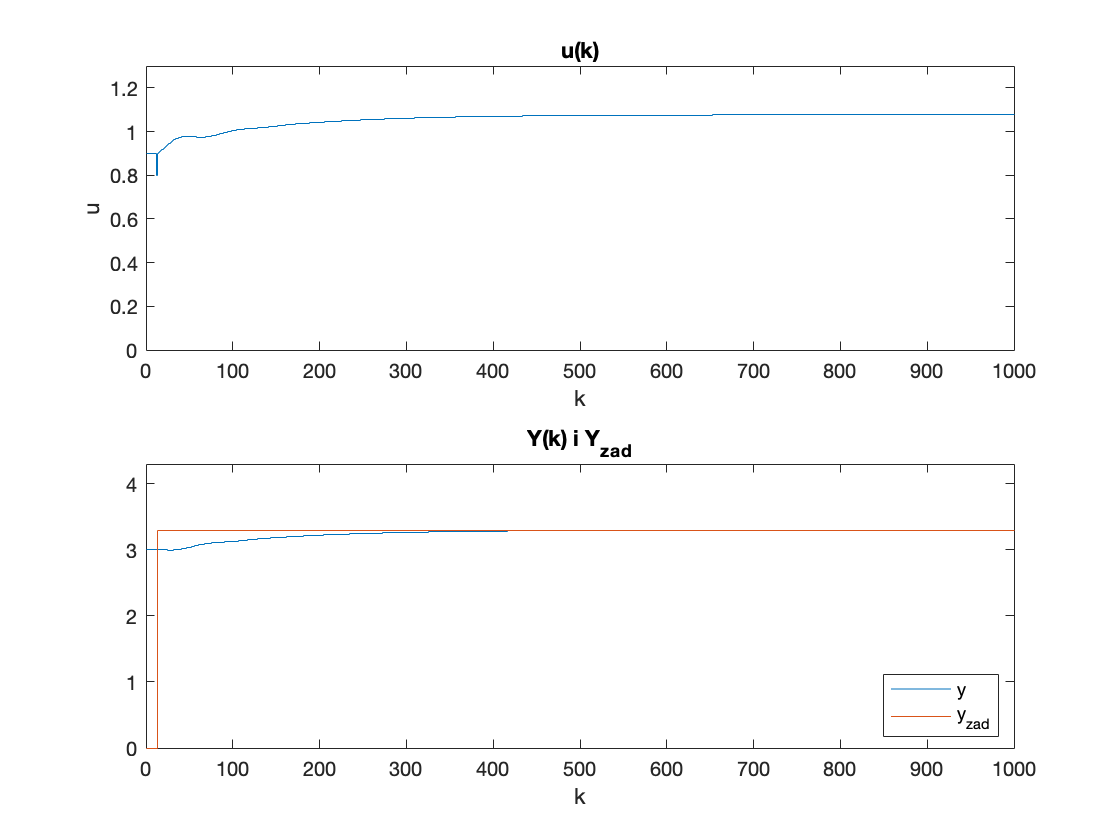
\includegraphics[scale=0.35]{png/pro_zad4_5_PID/pro1_PID_PI.png}
%	\caption{Regulator PI}
%	\label{rys_przebiegi_T1}
%\end{figure}

\begin{figure}[H]
	\centering
	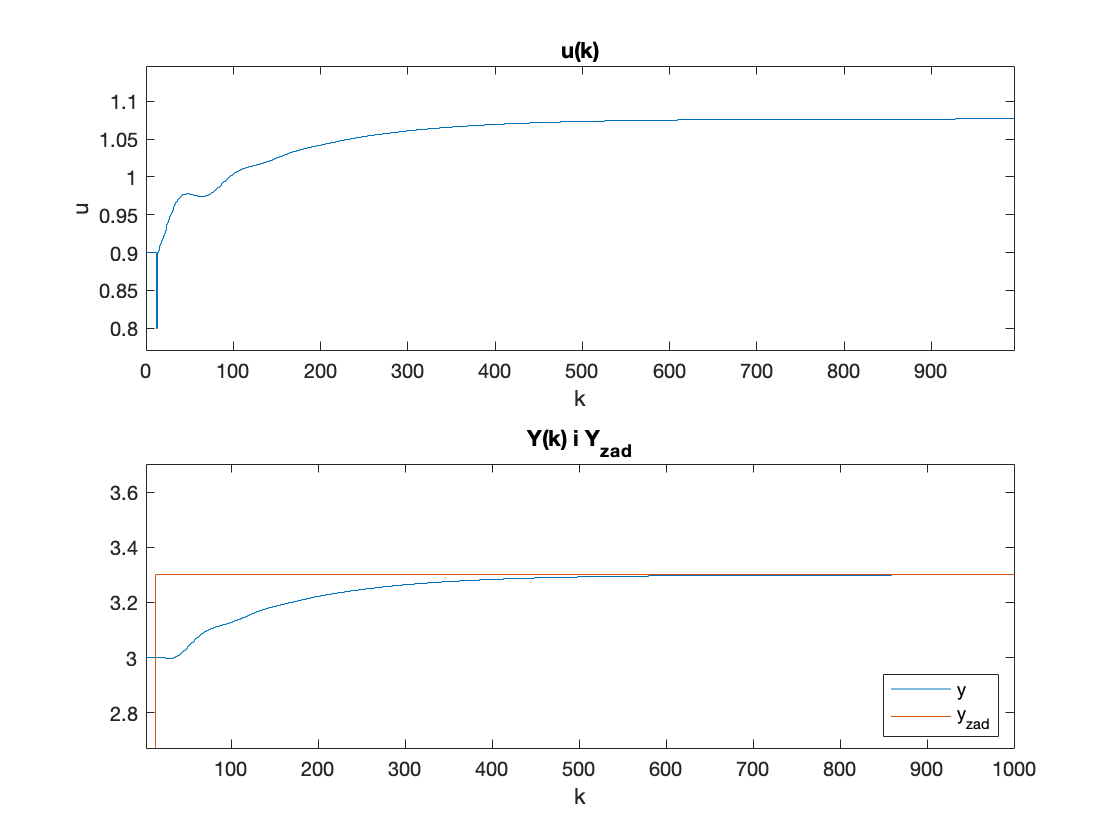
\includegraphics[scale=0.35]{png/pro_zad4_5_PID/pro1_PID_PI_zoomed.png}
	\caption{Regulator PI - przybli�ony}
	\label{rys_przebiegi_T1}
\end{figure}

PID ju� lepiej, ale nadal jest za wolny- stabilizuje si� dopiero dla k = 600

TO DO
Skoki dla regulatora PI

\begin{figure}[H]
	\centering
	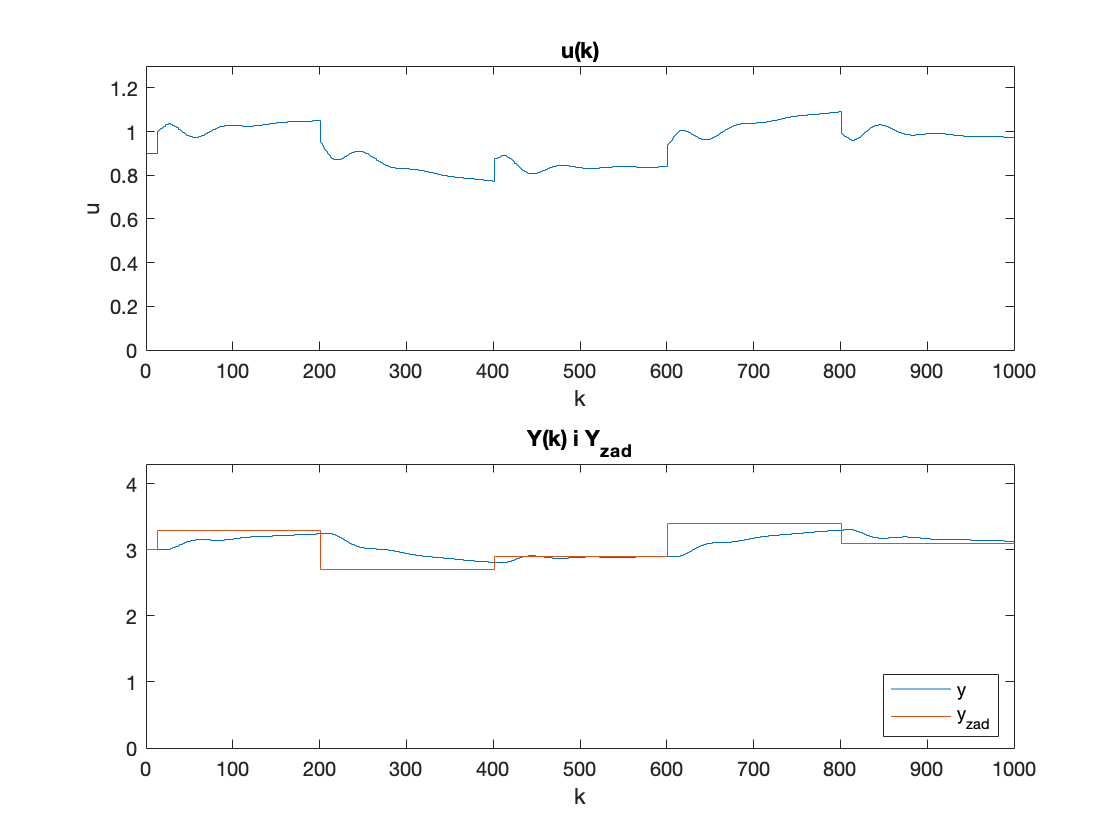
\includegraphics[scale=0.35]{png/pro_zad4_5_PID/pro1_PID_PI_skoki.png}
	\caption{Regulator PI - skoki}
	\label{rys_przebiegi_T1}
\end{figure}

Przy szybszych zmianach Y zad wida� �e PI jest zdecydowanie za wolny i nie nad��a za zmianami


TO DO
Nast�pnie wyznaczono nastawy dla regulatora PID

%\begin{figure}[H]
%	\centering
%	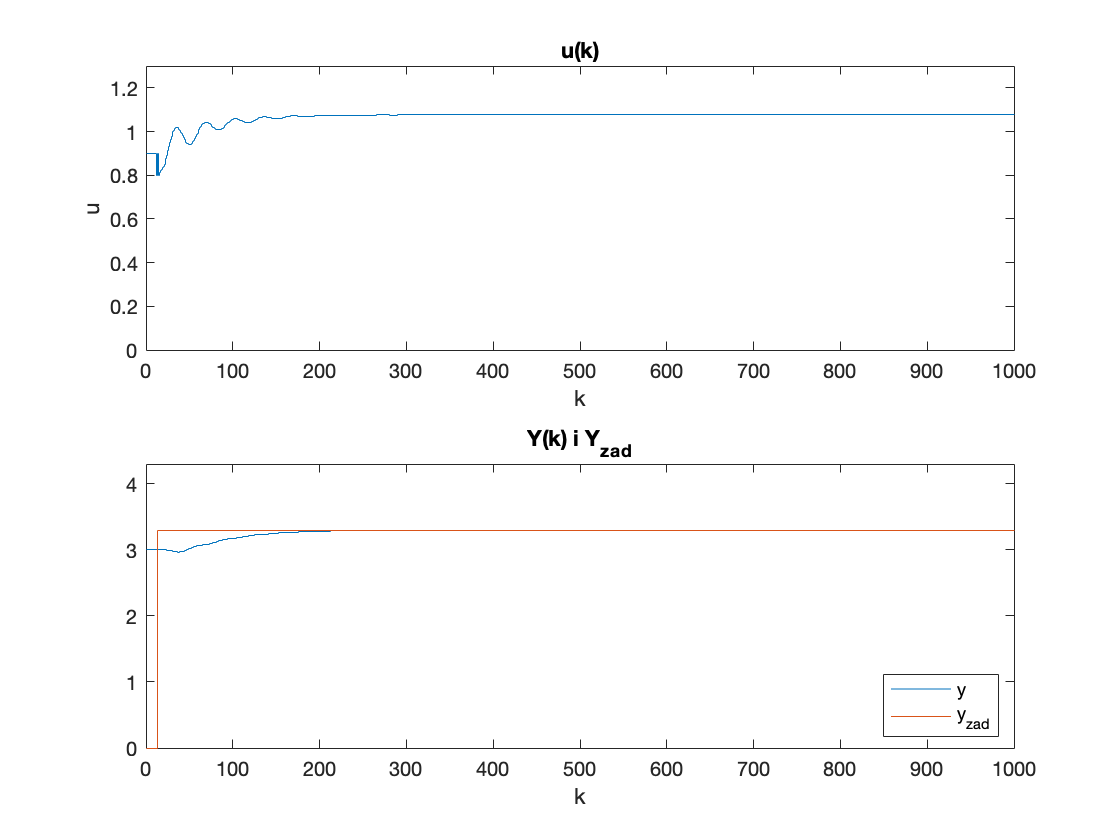
\includegraphics[scale=0.35]{png/pro_zad4_5_PID/pro1_PID_PID_niedostr.png}
%	\caption{Niedostrojony regulator PID}
%	\label{rys_przebiegi_T1}
%\end{figure}

\begin{figure}[H]
	\centering
	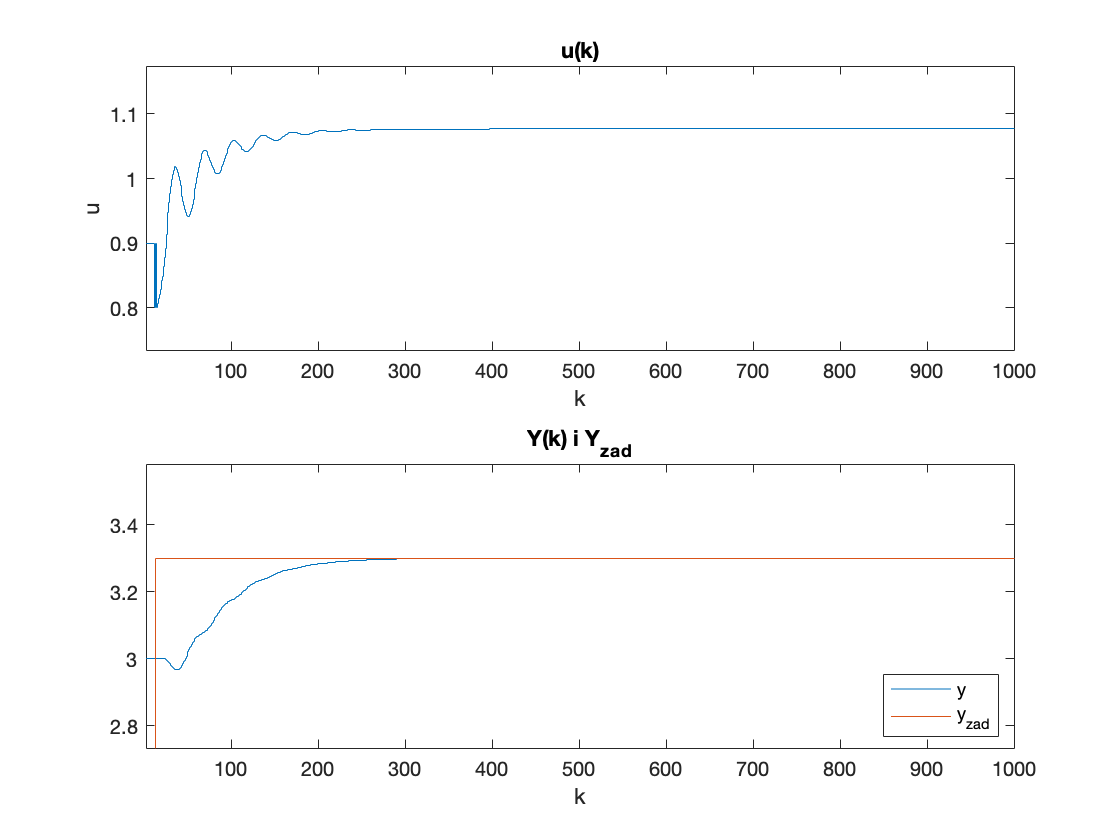
\includegraphics[scale=0.35]{png/pro_zad4_5_PID/pro1_PID_PID_niedostr_zoomed.png}
	\caption{Niedostrojony regulator PID - przybli�ony}
	\label{rys_przebiegi_T1}
\end{figure}

Skoki dla regulatora PID:

\begin{figure}[H]
	\centering
	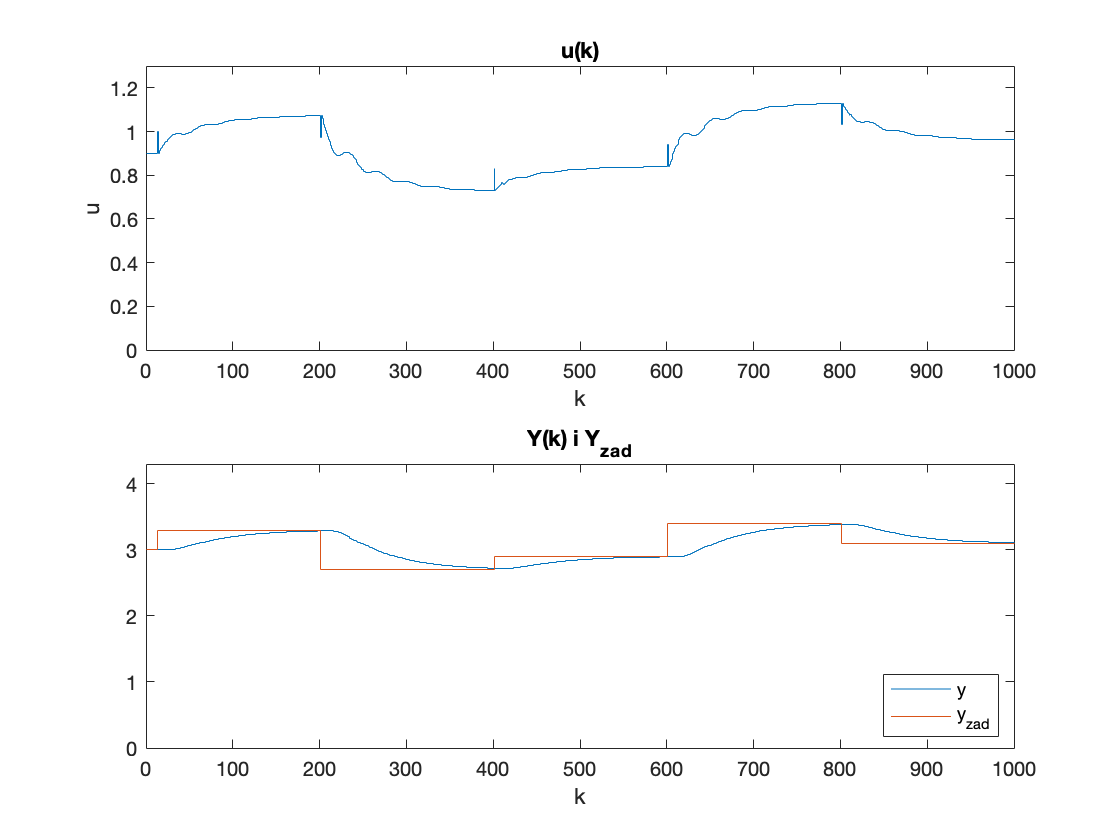
\includegraphics[scale=0.35]{png/pro_zad4_5_PID/pro1_PID_PID_niedostr_skoki.png}
	\caption{Niedostrojony regulator PID - skoki}
	\label{rys_przebiegi_T1}
\end{figure}

Nastawy regulatora PID dostrojono metod� eksperymentaln�.

\begin{figure}[H]
	\centering
	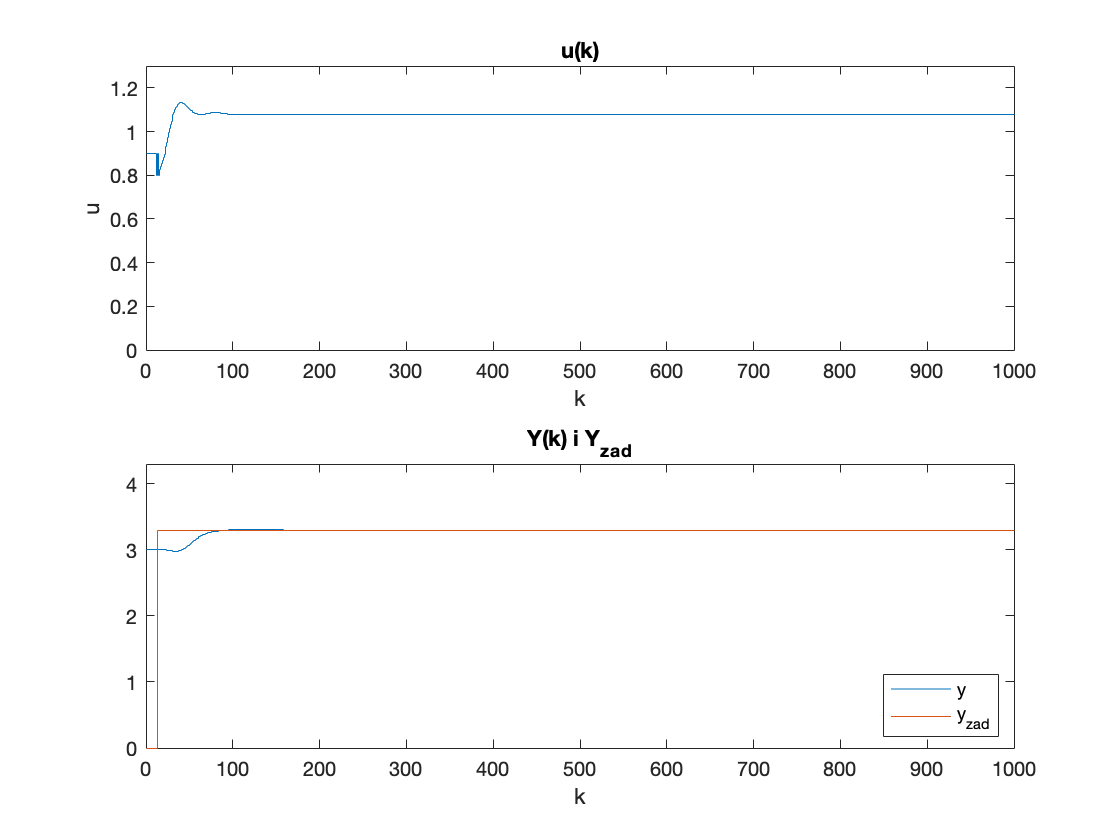
\includegraphics[scale=0.35]{png/pro_zad4_5_PID/pro1_PID_PID_dostr.png}
	\caption{Dostrojony regulator PID}
	\label{rys_przebiegi_T1}
\end{figure}

Skoki dla dostrojonego regulatora PID:

\begin{figure}[H]
	\centering
	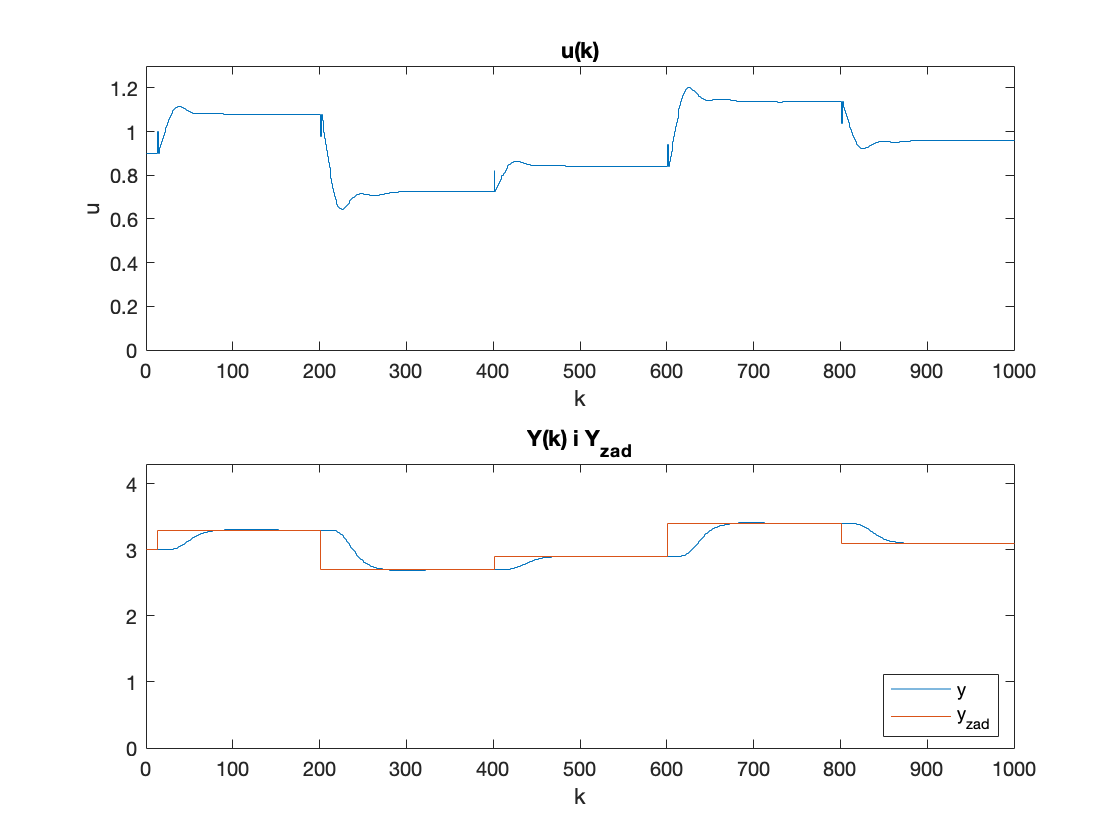
\includegraphics[scale=0.35]{png/pro_zad4_5_PID/pro1_PID_PID_dostr_skoki.png}
	\caption{Dostrojony regulator PID - skoki}
	\label{rys_przebiegi_T1}
\end{figure}


